\section{Auswertung}
\label{sec:Auswertung}

\subsection{Abstimmung des Probekopfes}
\label{sec:Abstimmung}
Der Schwingkreis wird auf eine Resonanzfrequenz von $\SI{46,223}{\mega\hertz}$
eingestellt und am Netzwerkanalysator ein Stehwellenverhältnis VSWR =
$\si{1,27}$ abgelesen. Damit ergibt sich nach:

\begin{equation}
    \text{VSWR} = \frac{\sqrt{P_{\text{T}}} + \sqrt{P_{\text{R}}}}
                {\sqrt{P_{\text{T}}} - \sqrt{P_{\text{R}}}}
    \iff
    P_{\text{R}} = \biggl( \frac{1-\text{VSWR}}{1+\text{VSWR}}^2 \biggr) \cdot P_{\text{T}}
\end{equation}

\noindent
eine reflektierende Leistung $P_{\text{R}}$ von circa $1,4\%$ der transmittierten
Leistung $P_{\text{T}}$. Die transmittierte Leistung $P_{\text{T}}$ beträgt etwa
$\SI{1}{\kilo\watt}$ und damit ergibt sich eine reflektierende Leistung
$P_{\text{R}} \approx \SI{14}{\watt}$

\subsection{Bestimmung der Phase}
\label{sec:phase}
In Abbildung \ref{fig:phase} ist der Reailteil der Signalintensität I($\varphi$) in Abhängigkeit
der Phase $\varphi$ für eine voll Periode dargestellt. Dabei wird eine maximale
Signalintensität von $185°$ (gestrichelte orangene Linie) gewählt.

\begin{figure}[H]
    \centering
    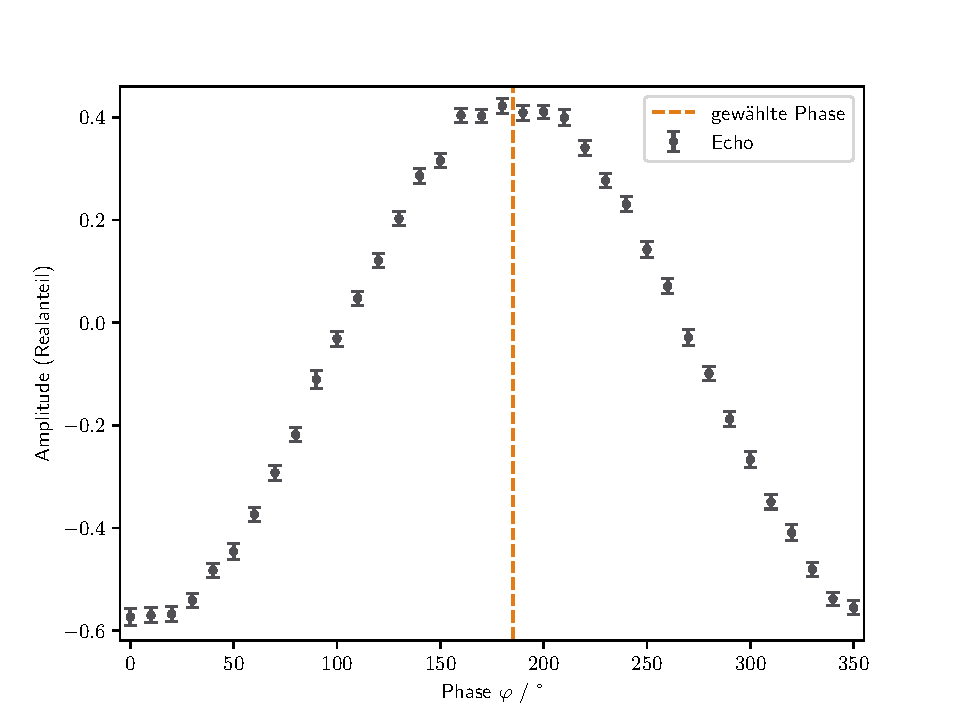
\includegraphics[width=0.8\textwidth]{Auswertung/winkel.pdf}
    \caption{Die Signalintensität I($\varphi$) in Abhängigkeit der Phase $\varphi$.
    Die für weitere Experimente gewähle Phase $\varphi$ ist in orange dargestellt.
    Die Signalintensität I($\varphi$) ist auf die Schwinungsbreite normiert.}
    \label{fig:phase}
\end{figure}

\subsection{Bestimmung der Pulslänge}
\label{sec:pulslaenge}
Um die Pulslänge $t_{\pi}$ des $180°$-Pulses zu bestimmen, wird die Singalintensität für
Pulsdauern von $\SI{1}{\micro\second}$ bis $\SI{20}{\micro\second}$ gemessen und das
Resultat in Abbildung \ref{fig:pulslaenge} aufgetragen. Eine maximale Singalintensität
ist bei einer Pulsdauer $t_{\pi} = \SI{5}{\micro\second}$ zu beobachten (siehe gestrichelte
orangene Linie in).

\begin{figure}[H]
    \centering
    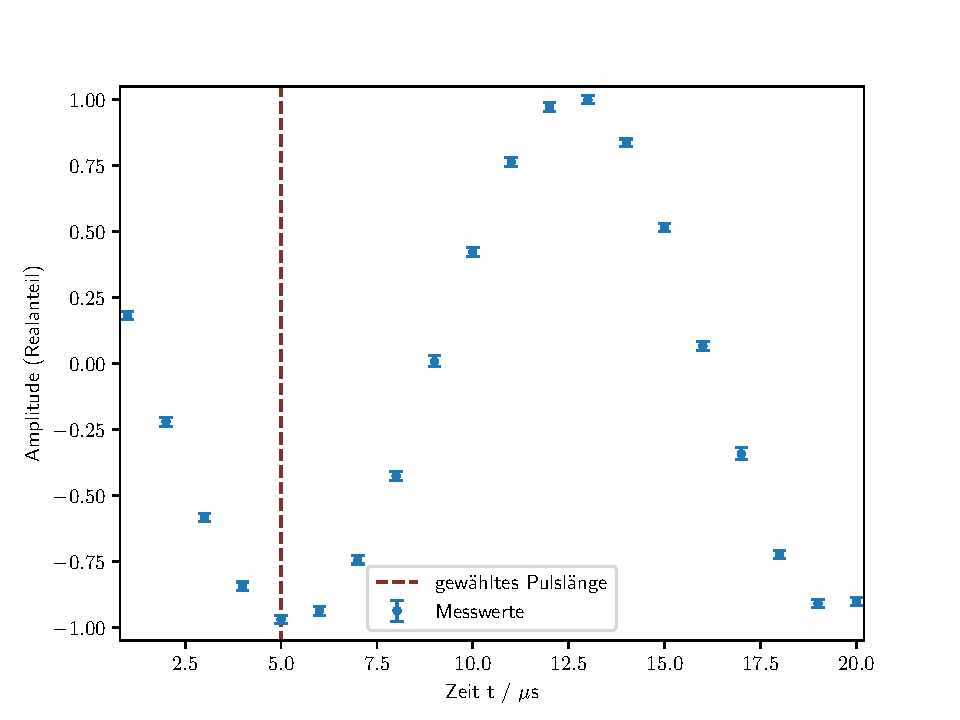
\includegraphics[width=0.8\textwidth]{Auswertung/pulslaenge.pdf}
    \caption{Die Signalintensität I($t_p$) in Abhängigkeit der Pulsdauer $t_{\text{p}}$. Die für weitere
    Experimente gewähle Pulsdauer $t_{\pi}$ ist in orange dargestellt. Die Signalintensität I($t_p$)
    ist auf die Schwinungsbreite normiert.}
    \label{fig:pulslaenge}
\end{figure}

\subsection{Bestimmung der Spin-Gitter Relaxationszeit $T_1$}
\label{sec:T1}
Zur Bestimmung der $T_1$-Zeit wird eine $\textit{saturation-recovery}$-Messung
durchgeführt. Die gemessene Signalintensität I(t) ist in Abbildung \ref{fig:T1}
aufgeführt. Mittels der Kohlrauschfunktion:
\begin{equation}
    I(t) = A \cdot \exp\biggl(-\left[\frac{t}{T_1} \right]^b
    \biggr) + B
\end{equation}
\noindent
kann die $T_1$-Zeit ermittelt werden. Es ergeben durch
$\textit{Python 3.7.6--scipy.optimize}$ sich dabei folgenden Parameter:
\begin{equation*}
  A = \SI{-0,984\pm0,006}{}
  \quad
  B = \SI{0,546\pm0,004}{}
  \quad
  b = \SI{0,546\pm0,004}{}
  \quad
  T_1 = \SI{18.313\pm0.350}{\milli\second}
\end{equation*}
\noindent

\begin{figure}[H]
    \centering
    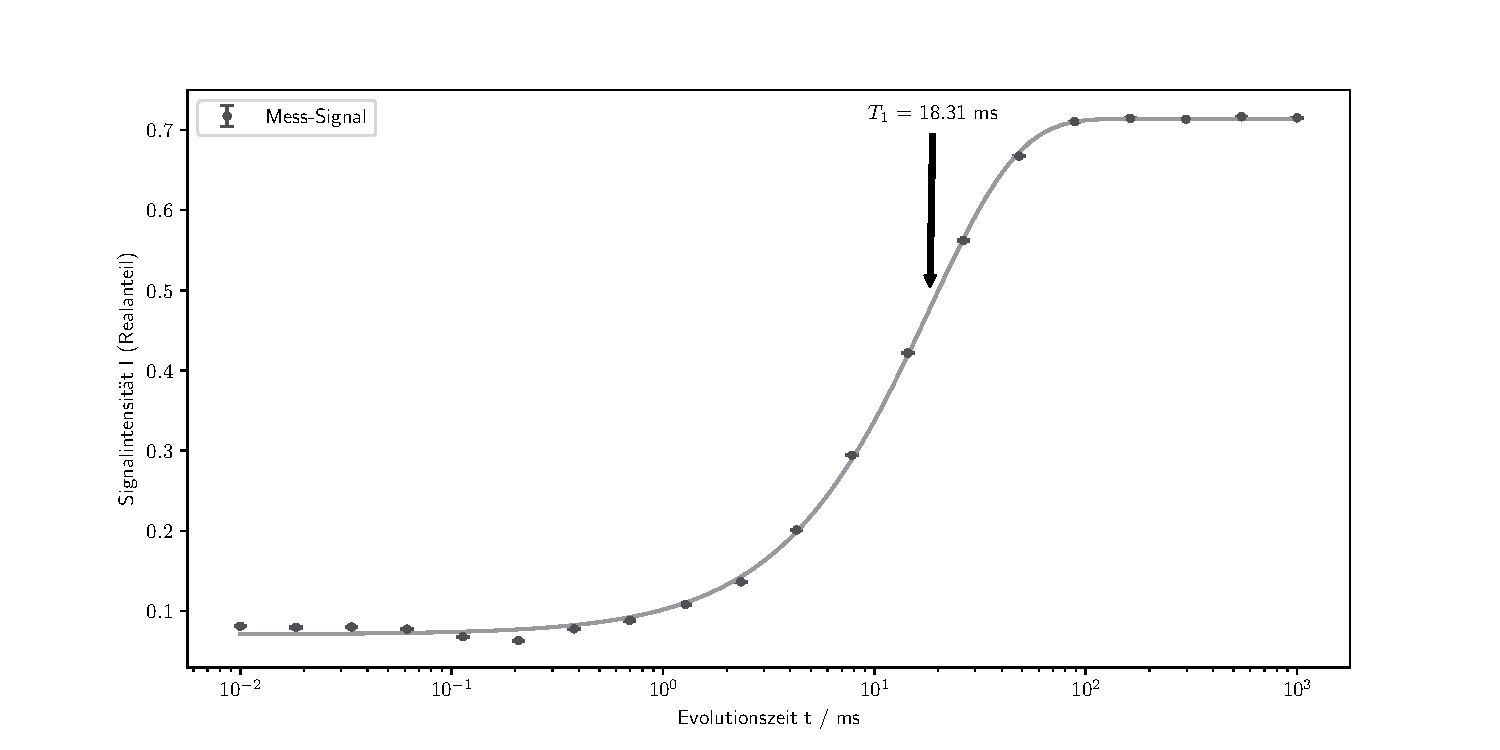
\includegraphics[width=\textwidth]{Auswertung/T1.pdf}
    \caption{$\textit{Saturation-recovery}$-Messung zu Bestimmung der Spin-Gitter
    Relaxationszeit. Die $T_1$-Zeit wird mittels einer Kohlrauschfunktion (hellgrau)
    ermittelt. Der Offset wird durch den Fitparameter $B$ korrigiert und die
    Singalintensität auf ihre Amplituden $A+B$ normiert.}
    \label{fig:T1}
\end{figure}

\subsection{Bestimmung der Spin-Spin Relaxationszeit $T_2$}
\label{sec:T2}
Um die $T_2$-Zeit zu ermitteln, wird die Signalintensität eines Festkörperecho
für Evolutionszeiten zwischen $\SI{20}{\micro\second}$ und $\SI{1}{\second}$
gemessen. Die Messung ist in Abbildung \ref{fig:T2} wieder zu finden.
Aus einer ähnlichen Kohlrauschfunktion, wie die in Unterkapitel \ref{sec:T1}
\begin{equation}
    I(t) = A \cdot \exp\biggl(-\left[\frac{2t}{T_2} \right]^b
    \biggr) + B
\end{equation}
\noindent
lässt die $T_2$-Zeit gewinnen. Dabei wird nun die Evolutionszeit $t$ zweifach gewählt,
da die transversale Magnetisierung zunächst dephasiert und durch den Echo-Puls
wieder rephasiert ($t_{\text{dep}}$ = $t_{\text{rep}} \rightarrow $ 2$t$).\\
Für die Kohlrausch-Parameter ergben sich mittels $\textit{Python 3.7.6--scipy.optimize}$
folgende Werte:
\begin{equation*}
  A = \SI{1,007\pm0,034}{}
  \quad
  B = \SI{-1,060\pm0,060}{}
  \quad
  b = \SI{-1,359\pm0,173}{}
  \quad
  T_2 = \SI{0.160\pm0.011}{\milli\second}
\end{equation*}

\begin{figure}[H]
    \centering
    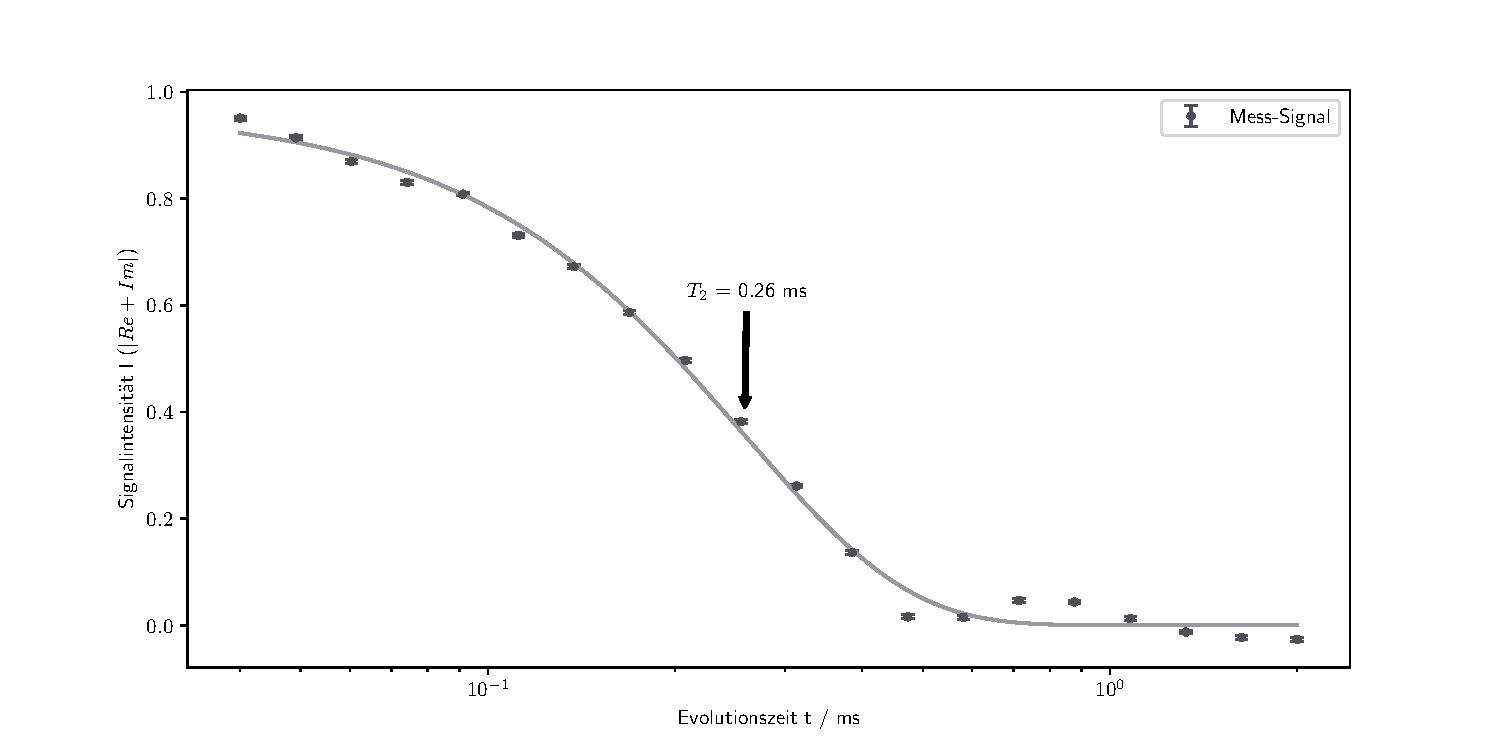
\includegraphics[width=\textwidth]{Auswertung/T2.pdf}
    \caption{$\textit{Saturation-recovery}$-Messung zu Bestimmung der Spin-Spin
    Relaxationszeit. Die $T_2$-Zeit wird mittels einer Kohlrauschfunktion (hellgrau)
    ermittelt. Der Offset wird durch den Fitparameter $B$ korrigiert und die
    Singalintensität auf ihre Amplituden $A+B$ normiert.}
    \label{fig:T2}
\end{figure}

\subsection{Messungen des stimulierten Echos}
\label{sec:stecho}
Das stimulierte Echo-Verfahren wird mit den Parametern $\varphi$ (Unterkapitel
\ref{sec:phase}), $t_{\pi}$ (Unterkapitel \ref{sec:pulslaenge}), $T_1$
(Unterkapitel \ref{sec:T1}) und $T_2$ (Unterkapitel \ref{sec:T2}) eingestellt.
Für eine feste Zeit $t_1$ von $\SI{25}{\micro\second}$ wird die transversale
Magnetisierung zunächst dephasieren
und die Signalintensität $I(t_{\text{m}})$ für unterschiedliche Mischzeiten
$t_{\text{m}}$ zwischen $\SI{20}{\micro\second}$ und $\SI{1}{\second}$ gemessen.
Die Magnetisierung ist unterteilt in einen $cos$-$cos$- und $sin$-$sin$-Anteil, welche
mittels zweier seperater Experimente untersucht werden. Die Messung des
$cos$-$cos$-Anteils ist in Abbildung \ref{fig:cos-cos}, und die des $sin$-$sin$-Anteils
in Abbildung \ref{fig:sin-sin} dargstellt.\\
Die $cos$-$cos$-Messung wird durch folgende Fit-Funktion genauer untersucht:
\begin{equation*}
  S(t) = S_0 + \biggl\{
  A \cdot \exp\biggl(-\left[\frac{t}{\tau_{\text{cos}}} \right]^{b_1}
  \biggr) + B
  \biggr\} \cdot
  \exp\biggl(-\left[\frac{t}{T_1} \right]^{b_2}
  \biggr)
\end{equation*}
\noindent,
mit der Korrelationszeit $\tau_{\text{cos}}$. Folgende Parameter ergeben sich
mittels $\textit{Python 3.7.6--scipy.optimize}$:
\begin{equation*}
  S_0 = \SI{-0.067\pm0.003}{}
  \quad
  A   = \SI{0.468\pm0.012}{}
  \quad
  B   = \SI{0.599\pm0.012}{}
  \quad
  b_1 = \SI{1,028\pm0,048}{}
\end{equation*}
\begin{equation*}
  b_2 = \SI{1,021\pm0.042}{}
  \quad
  \tau_{\text{cos}} = \SI{1,810\pm0,084}{\milli\second}
\end{equation*}

\begin{figure}[H]
    \centering
    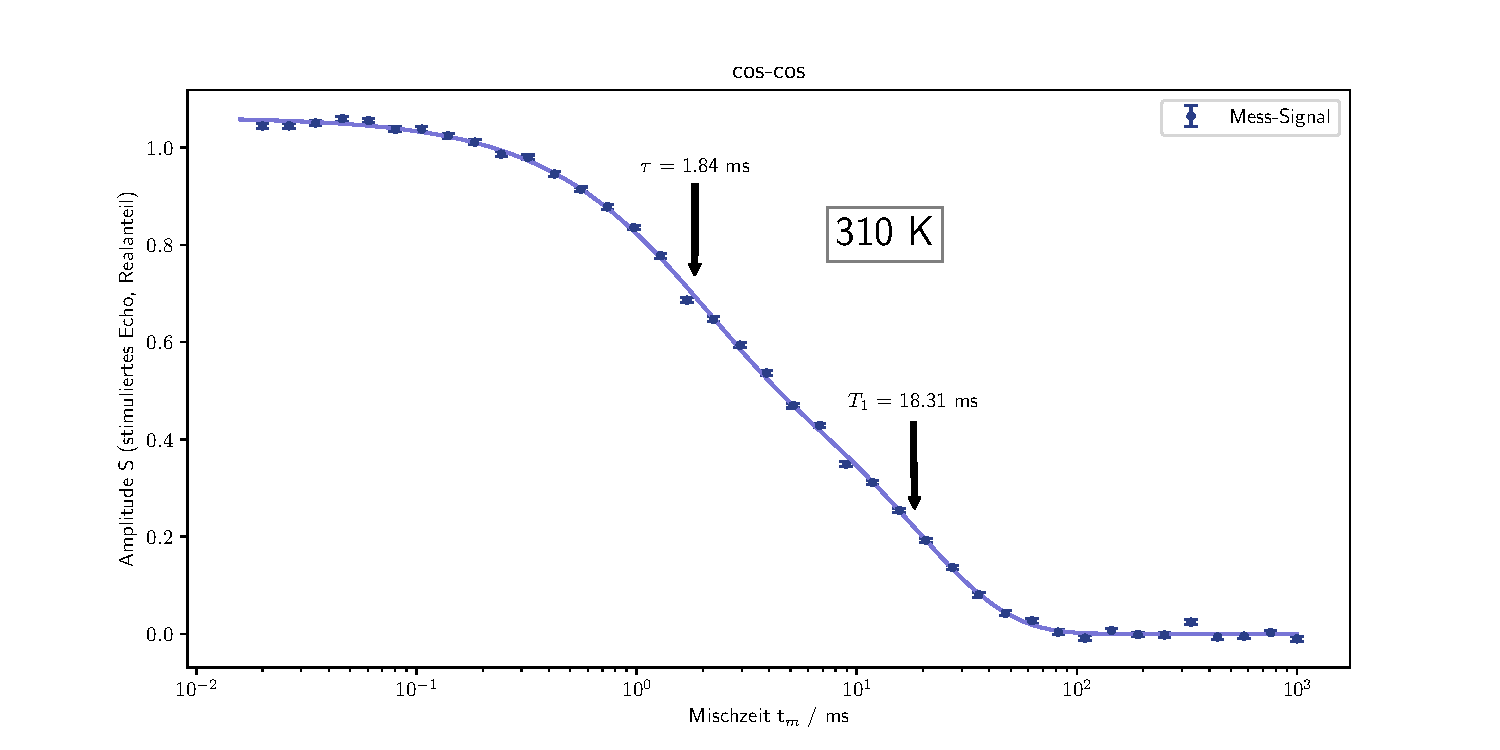
\includegraphics[width=\textwidth]{Auswertung/Para_der_Korrfkt/cos_cos.pdf}
    \caption{Stimulierte-Echo-Messung zu Bestimmung der Korrelationszeit
    $\tau_{\text{cos}}$. Die eingestellte $T_1$-Zeit, sowie die resultierende
    Korrelationszeit $\tau_{\text{cos}}$ ist durch die beiden Pfeile gekennzeichnet.
    Der Offset wird durch den Fitparameter $S_0$ korrigiert und die
    Singalintensität auf ihre Amplituden $S_0+A+B$ normiert.}
    \label{fig:cos-cos}
\end{figure}
\noindent
Die $sin$-$sin$-Messung wird mit der gleichen Fit-Funktion untersucht, nur das hier die $T_1$-Zeit nun auch als Parameter $T_{1,Q}$ freigegeben wird:
\begin{equation*}
  S(t) = S_0 + \biggl\{
  A \cdot \exp\biggl(-\left[\frac{t}{\tau_{\text{sin}}} \right]^{b_1}
  \biggr) + B
  \biggr\} \cdot
  \exp\biggl(-\left[\frac{t}{T_{1,Q}} \right]^{b_2}
  \biggr)
\end{equation*}
\noindent
$\textit{Python 3.7.6--scipy.optimize}$ gibt dabei folgende Parameter wieder:
\begin{equation*}
  S_0 = \SI{-0.080\pm0.010}{}
  \quad
  A   = \SI{0.589\pm0.037}{}
  \quad
  B   = \SI{0.491\pm0.024}{}
  \quad
  b_1 = \SI{1,119\pm0.148}{}
\end{equation*}
\begin{equation*}
  b_2 = \SI{0,907\pm0,113}{}
  \quad
  \tau_{\text{sin}} = \SI{0,253\pm0,019}{\milli\second}
  \quad
  T_{1,Q} = \SI{42,754\pm3,911}{\milli\second}
\end{equation*}

\begin{figure}[H]
    \centering
    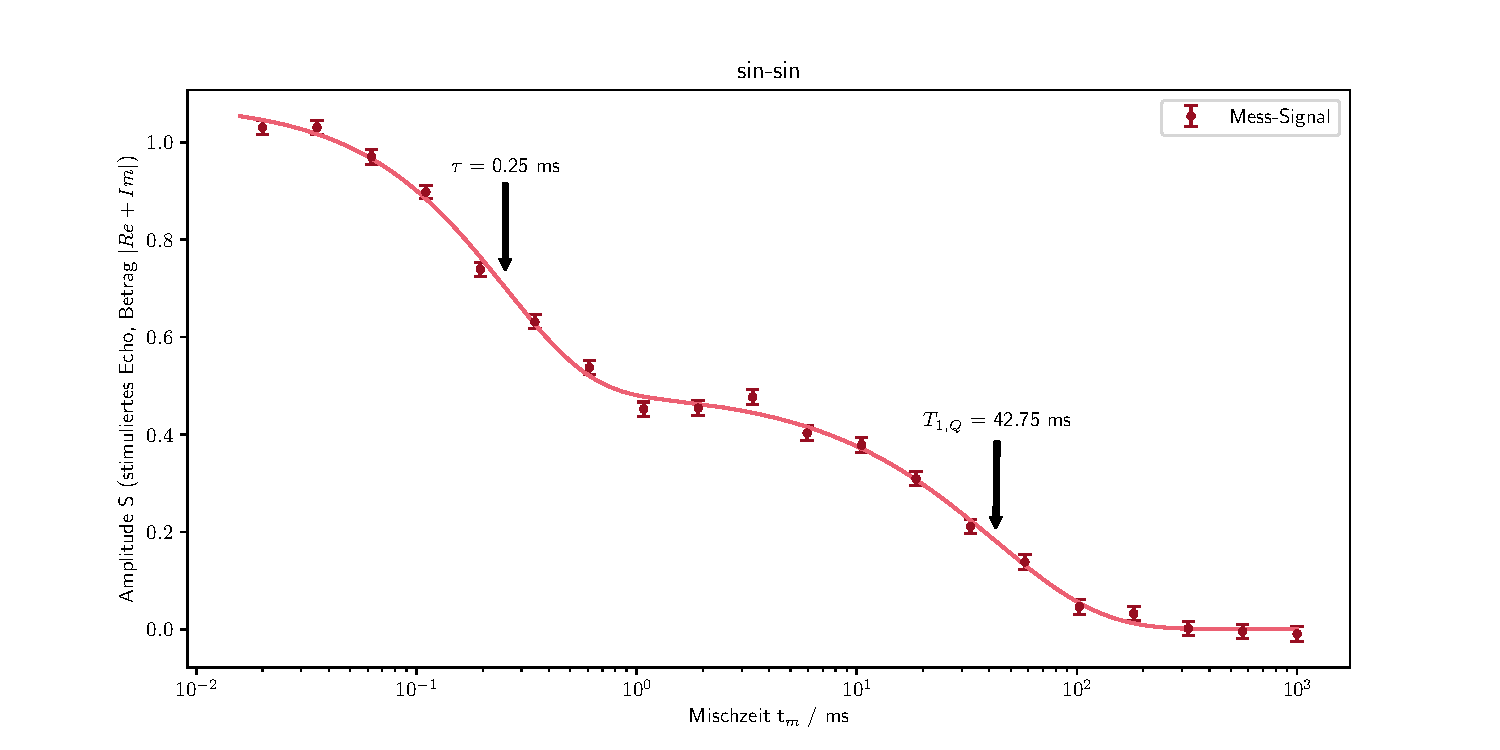
\includegraphics[width=\textwidth]{Auswertung/Para_der_Korrfkt/sin_sin.pdf}
    \caption{Stimulierte-Echo-Messung zu Bestimmung der Korrelationszeit
    $\tau_{\text{sin}}$. Die eingestellte $T_1$-Zeit, sowie die resultierende
    Korrelationszeit $\tau_{\text{sin}}$ ist durch die beiden Pfeile gekennzeichnet.
    Der Offset wird durch den Fitparameter $S_0$ korrigiert und die
    Singalintensität auf ihre Amplitude $S_0+A+B$ normiert.}
    \label{fig:sin-sin}
\end{figure}

\subsection{Temperaturabhängigkeit}
\label{sec:tempabh}
Analog zu der Messung aus dem Unterkapitel \ref{sec:stecho}, wird nun die
Korrelationszeit $\tau$ Temperaturen zwischen $\SI{310}{\kelvin}$
und $\SI{346}{\kelvin}$ bestimmt. In Abbildung \ref{fig:korrtemp}
ist die Korrelationszeit $\tau$ der $cos$-$cos$- und $sin$-$sin$-Messungen
in Abhängigkeit der Temperatur aufgetragen. Die Korrelationszeit folgt
dem Arrhenius-Gesetz $\tau = \tau_0 \exp{E/k_{\text{B}}T}$, sodass man den Messwerten
folgende Ausgleichsgerade anlegt:
\begin{equation*}
  \ln{\tau} = m \cdot \frac{1}{T} + b
\end{equation*}
\noindent
und damit die Aktivierungsenergie $E$ = m $\cdot k_{\text{B}}$ und den Vorfaktor $\tau_0 = \exp{(b)}$ erhält. Es ergeben sich mittels
$\textit{Python 3.7.6--scipy.optimize}$ folgende Werte:
\begin{equation*}
  \text{m}_{\text{cos}} = \SI{10588,585\pm594,569}{\kelvin}
  \quad\rightarrow\quad
  E = \SI{0.912\pm0.051}{\electronvolt}
\end{equation*}
\begin{equation*}
  \text{b}_{\text{cos}} = \SI{-33,536\pm1,816}
  \quad\rightarrow\quad
  \tau_0 = \SI{27,258\pm0.012 e-13}{\second}
\end{equation*}
\begin{equation*}
  \text{m}_{\text{sin}} = \SI{9641,512\pm140,781}{\kelvin}
  \quad\rightarrow\quad
  E = \SI{0.831\pm0.012}{\electronvolt}
\end{equation*}
\begin{equation*}
  \text{b}_{\text{sin}} = \SI{-30,597\pm0.430}
  \quad\rightarrow\quad
  \tau_0 = \SI{515,100\pm0.012 e-13}{\second}
\end{equation*}

\begin{figure}[H]
    \centering
    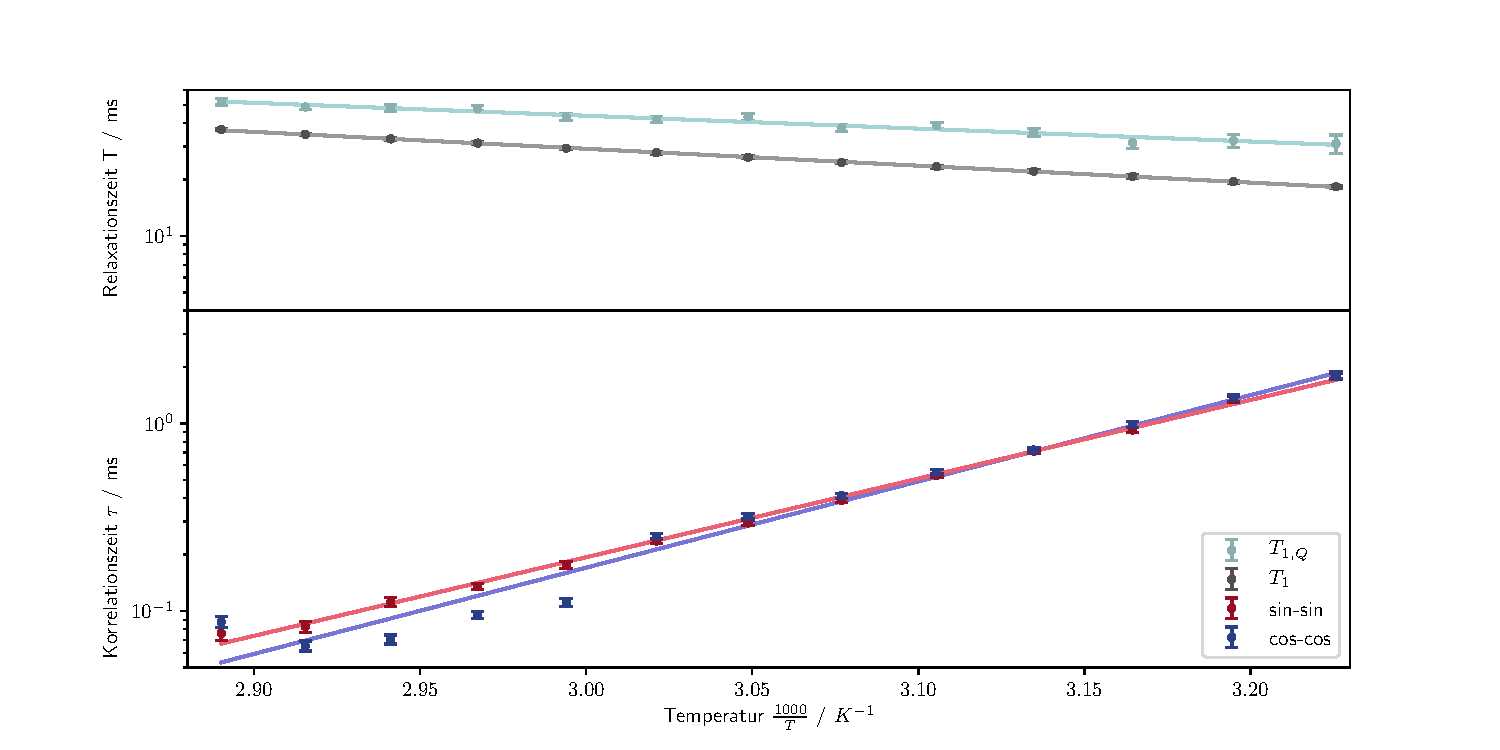
\includegraphics[width=\textwidth]{Auswertung/Tempabh/Korr_Temp.pdf}
    \caption{}
    \label{fig:tempabh}
\end{figure}


\begin{figure}[H]
    \centering
    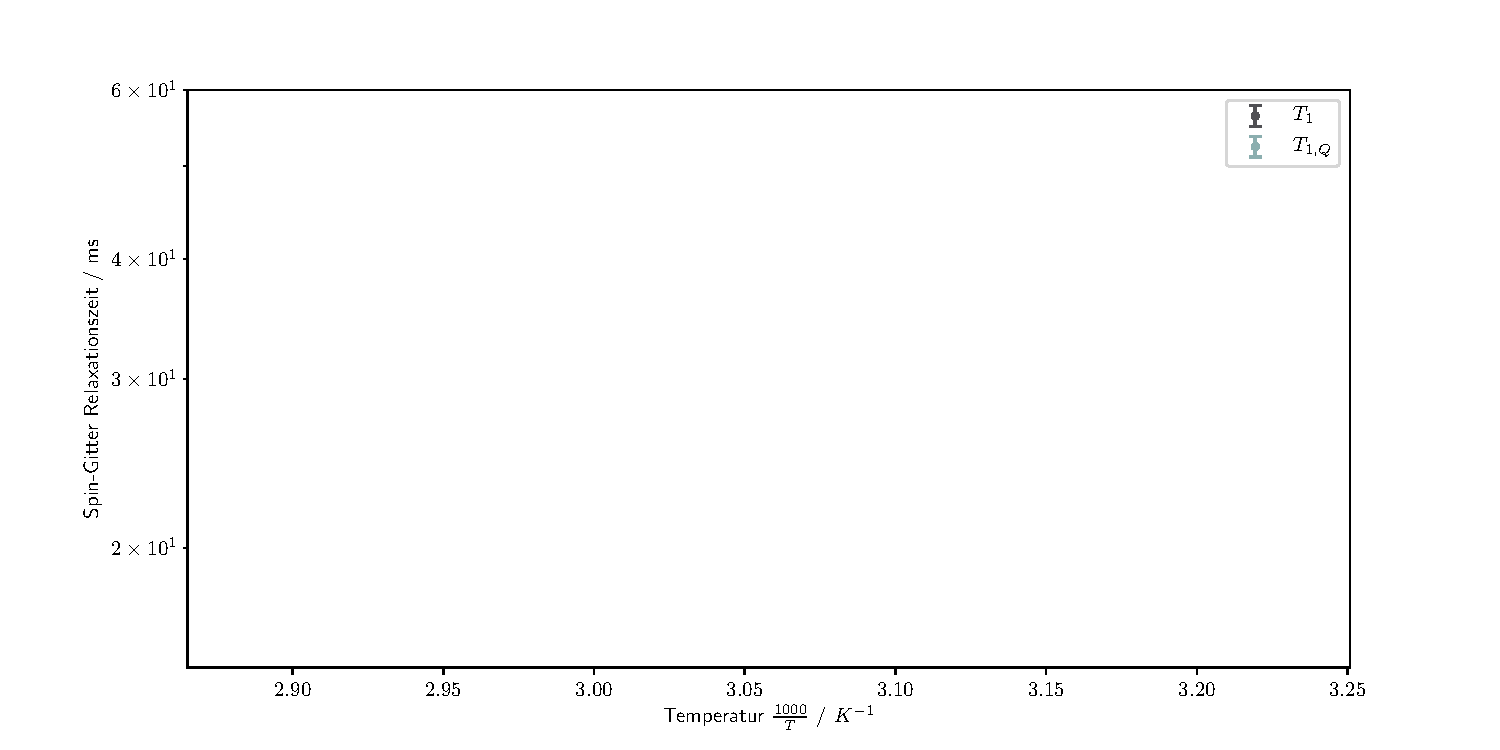
\includegraphics[width=\textwidth]{Auswertung/Tempabh/T1.pdf}
    \caption{}
    \label{fig:t1t1q}
\end{figure}
